\section{Architecture}

The size of the log files which PET has to parse can easily be 10s of gigabytes
large, thus PET has to be designed with performance in mind. It is not feasible
to read the entire log file into memory and then start parsing, as it would
probably exhaust the memory of most current workstations. It will also be a bad
idea to read one line, parse it, weight it and apply it to the grand total, as
it would not be able to utilize the power of multi core processors. For speed,
PET is built using ideas from the producer-consumer scheme as explained by Gamma
et. al. in\cite{designpatterns}.

The process of reading the log file is difficult to run with multiple threads, but
with some clever thoughts, it is rather easy to let a producer read the lines into a ring buffer
and pick from this ring buffer using multiple consumers. Each consumer parses the log lines
they pick, and apply the events to each their result vector. When all lines are read and parsed,
the results vectors are merged, and idle-task power and static power consumption is added.

\autoref{fig:callgraph}


PET is a tool which main task will be to 

When designing a tool for parsing large input files and applying flexible configuration alternatives,
there are quite a few aspects that needs to be considered. Through this section the design choises
briefly explained in \autoref{sec:whatispet} will be further explained and more deeply understood.

PET has to be designed for good performance.


\begin{figure}
    \includegraphics[width=0.9\textwidth]{figs/pet-pipeline-gv.pdf}
    \caption{How PET works}
    \label{fig:pipeline}
\end{figure}

\begin{figure}
%    \includesvg[clean,eps,pretex=\relscale{0.25},width=\textwidth]{figs/maincallgraph}
    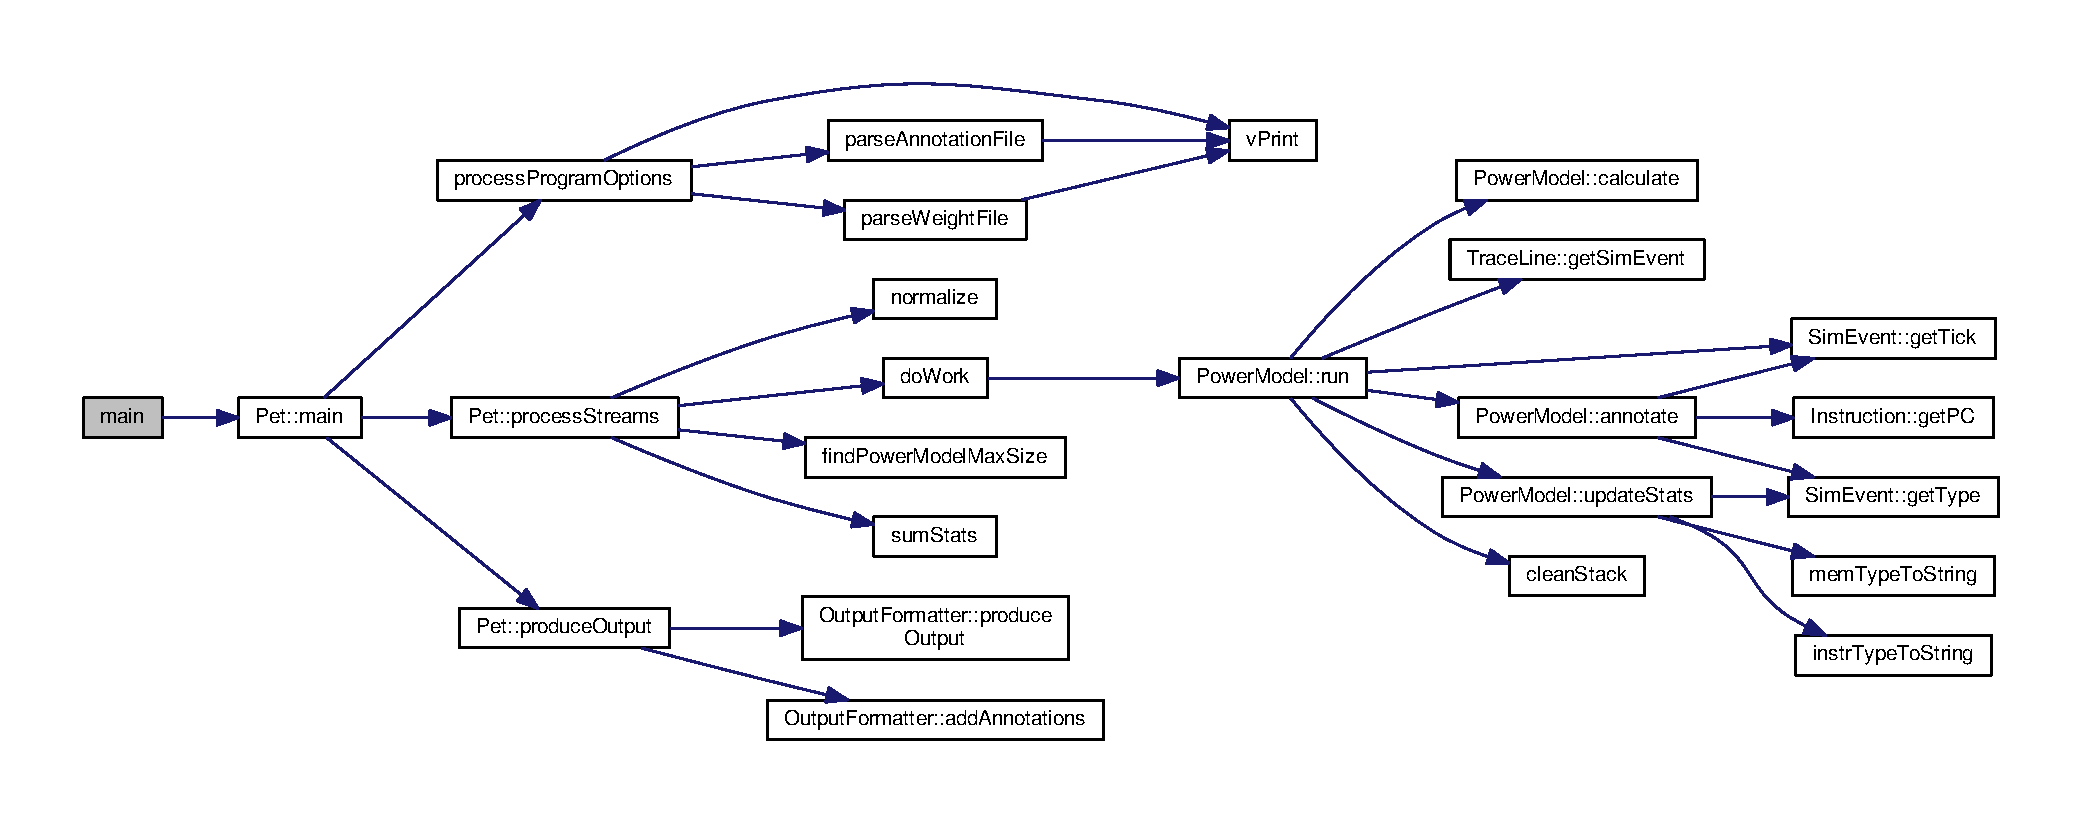
\includegraphics[width=\textwidth]{figs/maincallgraph.pdf}
    \caption{Call graph}
    \label{fig:callgraph}
\end{figure}

put UML-figures here
trådpool
concurency
arbeidsdeling
ringbuffer, statisk vs. ikke statis størrelse




